\documentclass[../thesis.tex]{subfiles}

\begin{document}

\chapter{Introduction}
\section{Motivation}
\lettrine{R}{obots} are awesome. \blindtext
Here's a citation \cite{jackson_ALTROC_2021a}. \blindtext And another 
citation \cite{jacksonPerformanceDynamicallySimulated2016}.

\begin{figure}[t]
    \centering
    \begin{subfigure}[b]{0.24\columnwidth}
        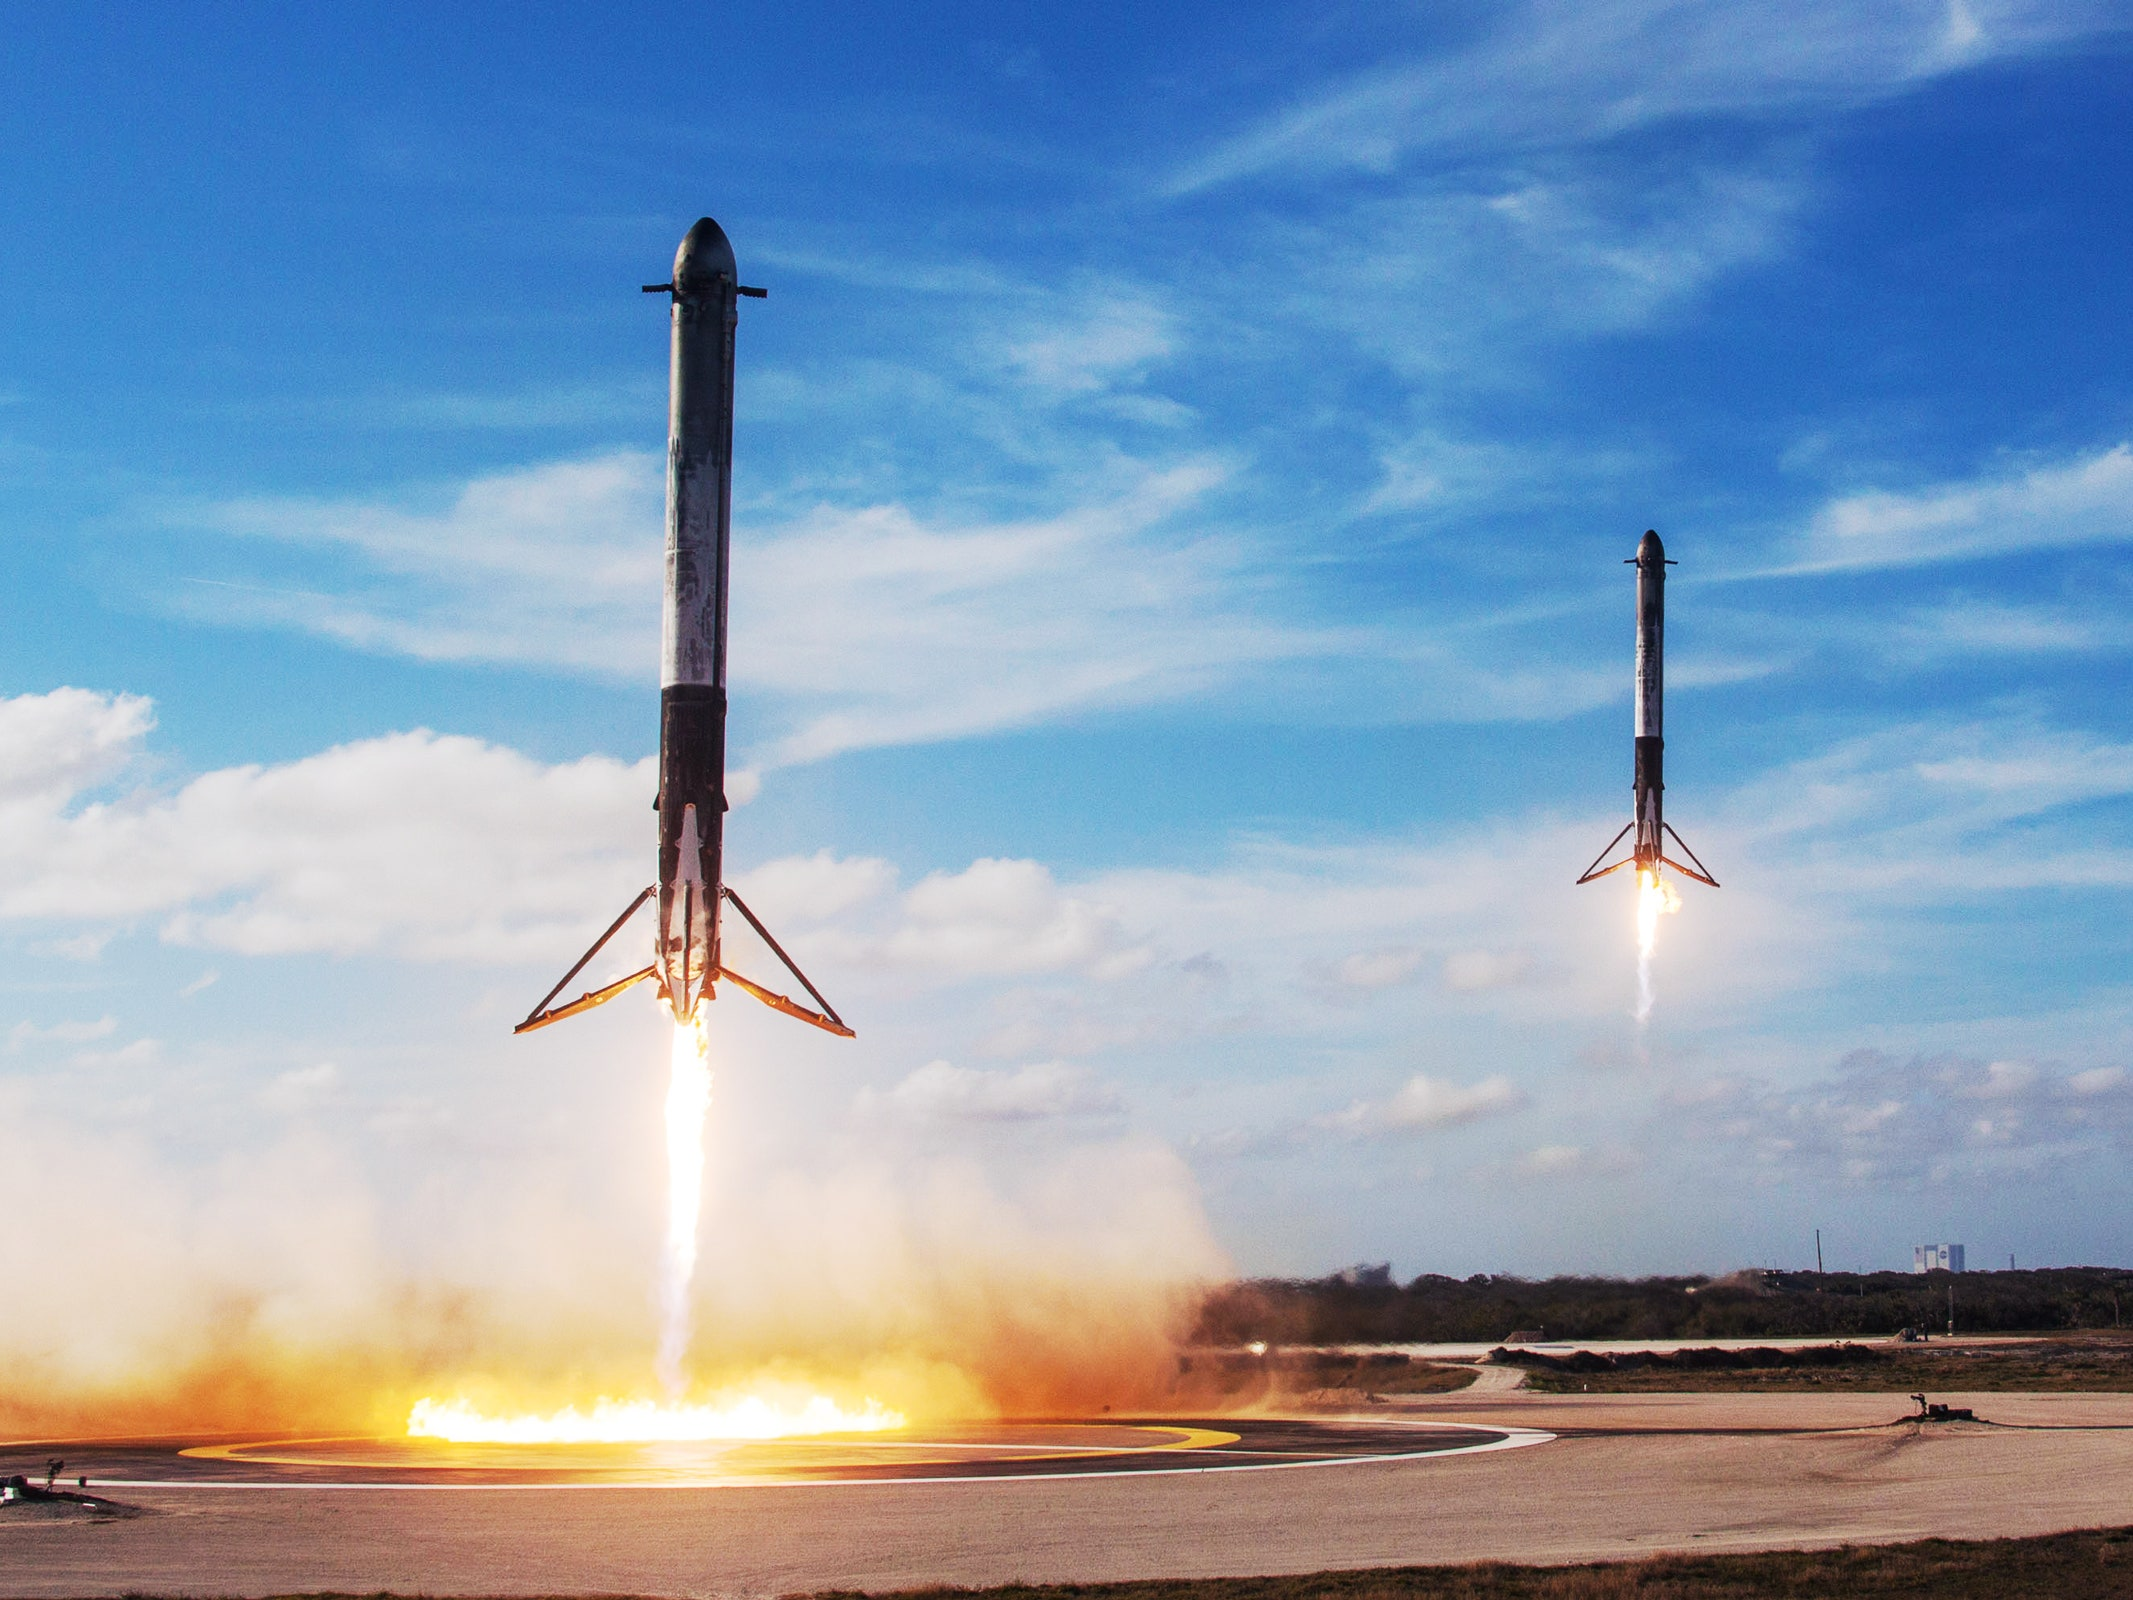
\includegraphics[height=0.8\textwidth, trim=3cm 0 3cm 0, clip]{spacexrocketreturn.jpg} 
        \caption{}
    \end{subfigure}
    \begin{subfigure}[b]{0.24\columnwidth}
        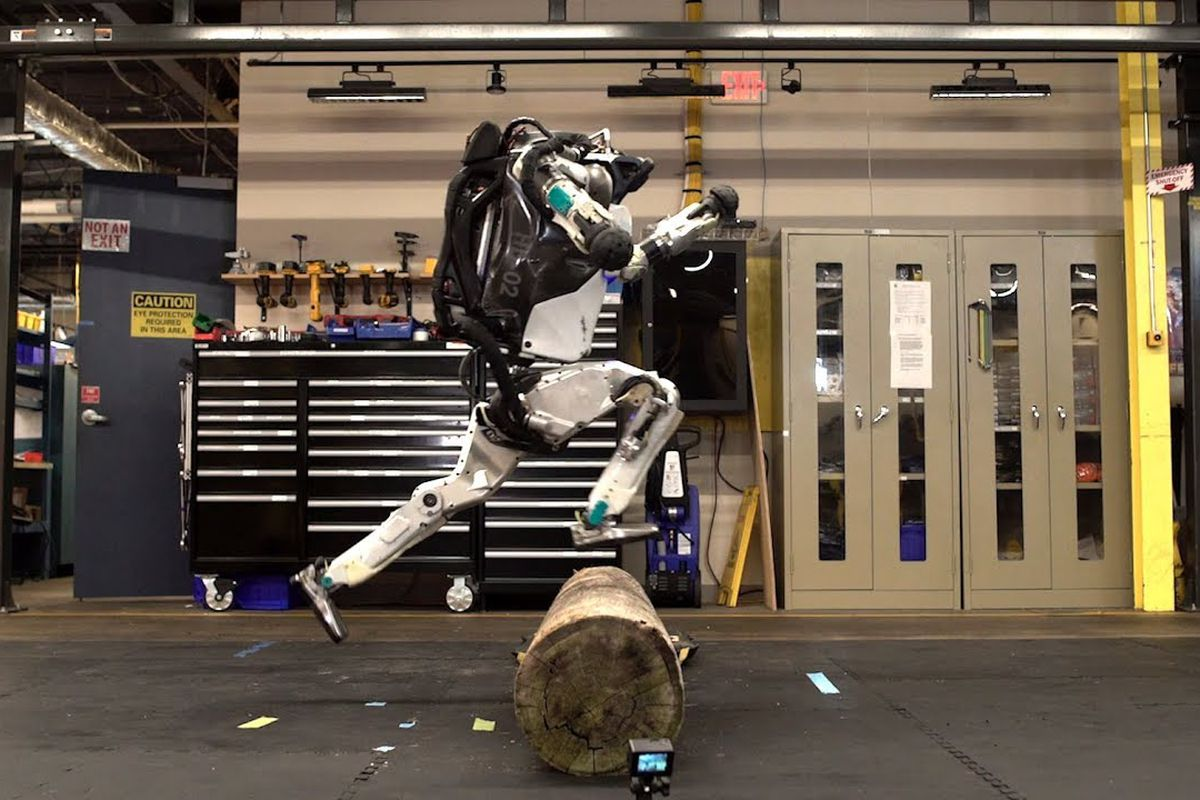
\includegraphics[height=0.8\textwidth, trim=4cm 0 4cm 0, clip]{atlas.jpg} 
        \caption{}
    \end{subfigure}
    \begin{subfigure}[b]{0.24\columnwidth}
        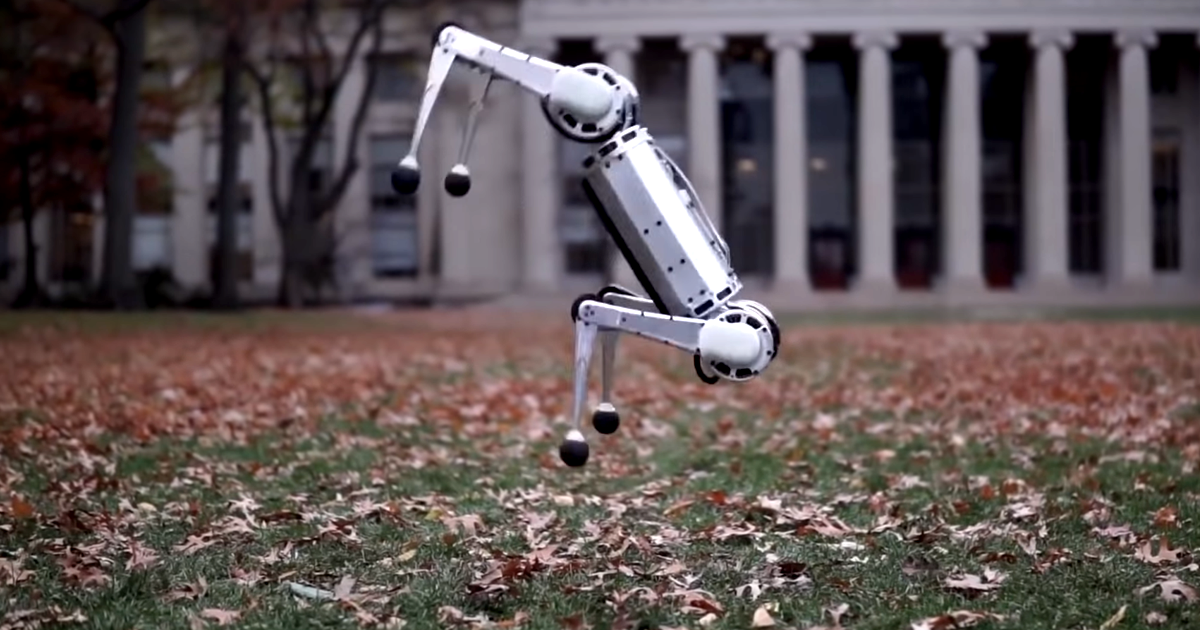
\includegraphics[height=0.8\textwidth, trim=8cm 0 8cm 0, clip]{mini-cheetah-robot-bloopers.png} 
        \caption{}
    \end{subfigure}
    \begin{subfigure}[b]{0.24\columnwidth}
        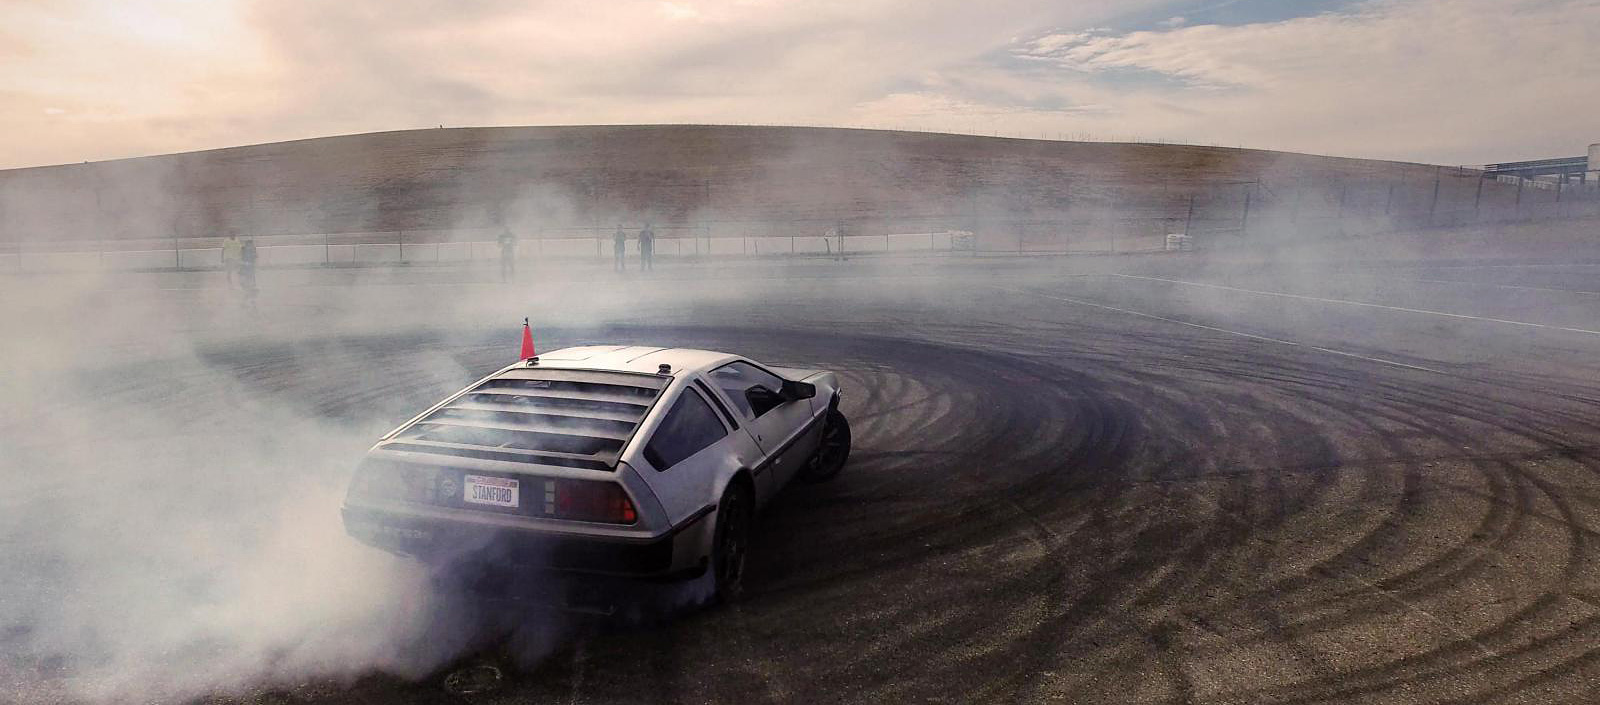
\includegraphics[height=0.8\textwidth, trim=100 0 400 0, clip]{Stanford_MARTY_005_remasted-banner.jpg} 
        \caption{}
    \end{subfigure}
    \caption{Notable recent successes of optimal control, a) SpaceX rocket booster landing (2018), b) Boston Dynamics' Atlas doing parkour (2018), c) MIT Mini Cheetah doing backflips (2019), and d) Stanford's MARTY drifing around a racecourse (2019).}
    \label{fig:applications}
\end{figure}

\blindtext[3]


\section{Key Challenges} 

\blindtext

\section{Contributions}

\blinditemize

\section{Outline}

\blindtext[3]

\end{document}